\subsection{Internal classification and \texorpdfstring{$S_\mathrm{RG}$}{S\_RG} evaluation}
\label{sec:results_internal}

The internal results summarise the ensemble predictions across the full LoTSS-DR2 sample. Class membership, confidence and agreement are presented first, followed by the distributions of the similarity-score components and membership in the adopted score bands.

\subsubsection{Ensemble classification catalogue}
\label{sec:results_classification}

The ensemble classification catalogue contains \(32\,514\) sources across eleven morphology classes (Table~\ref{tab:classification_catalogue}). Edge-bright FRII and Structured-Bent are the most common assignments, together accounting for \(45.4\,\%\) of the sample, whereas Amorphous sources constitute only \(1.2\,\%\). These are predicted image-morphology groups, rather than independently confirmed physical source populations.

Bright-core sources have the highest mean confidence, while Amorphous and Asymmetric core-jet sources have the lowest (Table~\ref{tab:classification_catalogue}). Confidence and agreement describe the concentration and consistency of predictions, rather than classification accuracy. Figure~\ref{fig:classification_confidence_extremes} compares the most and least confident assignments within each class.

The ensemble correctly classifies \(28\) of the \(33\) test images withheld from supervised training (\(84.8\,\%\)). Most errors involve ACJ and Structured-Bent sources (Table~\ref{tab:heldout_counts}). With only three examples per class and prior exposure during pre-training, this test provides limited evidence of performance on new survey sources.

\begin{table}[H]
\centering
\small
\begin{tabular}{lrrrr}
\toprule
Class & Count & Fraction & Confidence & Agreement \\
\midrule
Amorphous & 390 & 1.2\,\% & 0.651 & 0.869 \\
Asymmetric core-jet (ACJ) & 1\,976 & 6.1\,\% & 0.660 & 0.894 \\
Bright-core & 3\,728 & 11.5\,\% & 0.865 & 0.946 \\
Centre-bright (FRI) & 3\,323 & 10.2\,\% & 0.785 & 0.912 \\
Core-Displaced & 980 & 3.0\,\% & 0.697 & 0.834 \\
Edge-bright (FRII) linear & 7\,574 & 23.3\,\% & 0.821 & 0.931 \\
Hybrid (FRX) unclear & 2\,865 & 8.8\,\% & 0.718 & 0.909 \\
Large FRII & 2\,425 & 7.5\,\% & 0.774 & 0.876 \\
Spirals & 963 & 3.0\,\% & 0.756 & 0.907 \\
Structured-Bent & 7\,197 & 22.1\,\% & 0.740 & 0.918 \\
Unresolved & 1\,093 & 3.4\,\% & 0.711 & 0.873 \\
\midrule
Total & 32\,514 & 100\,\% & & \\
\bottomrule
\end{tabular}
\caption[Class composition, confidence and agreement]{Class composition and mean ensemble confidence and agreement.}
\label{tab:classification_catalogue}
\end{table}

\begin{figure}[H]
\centering
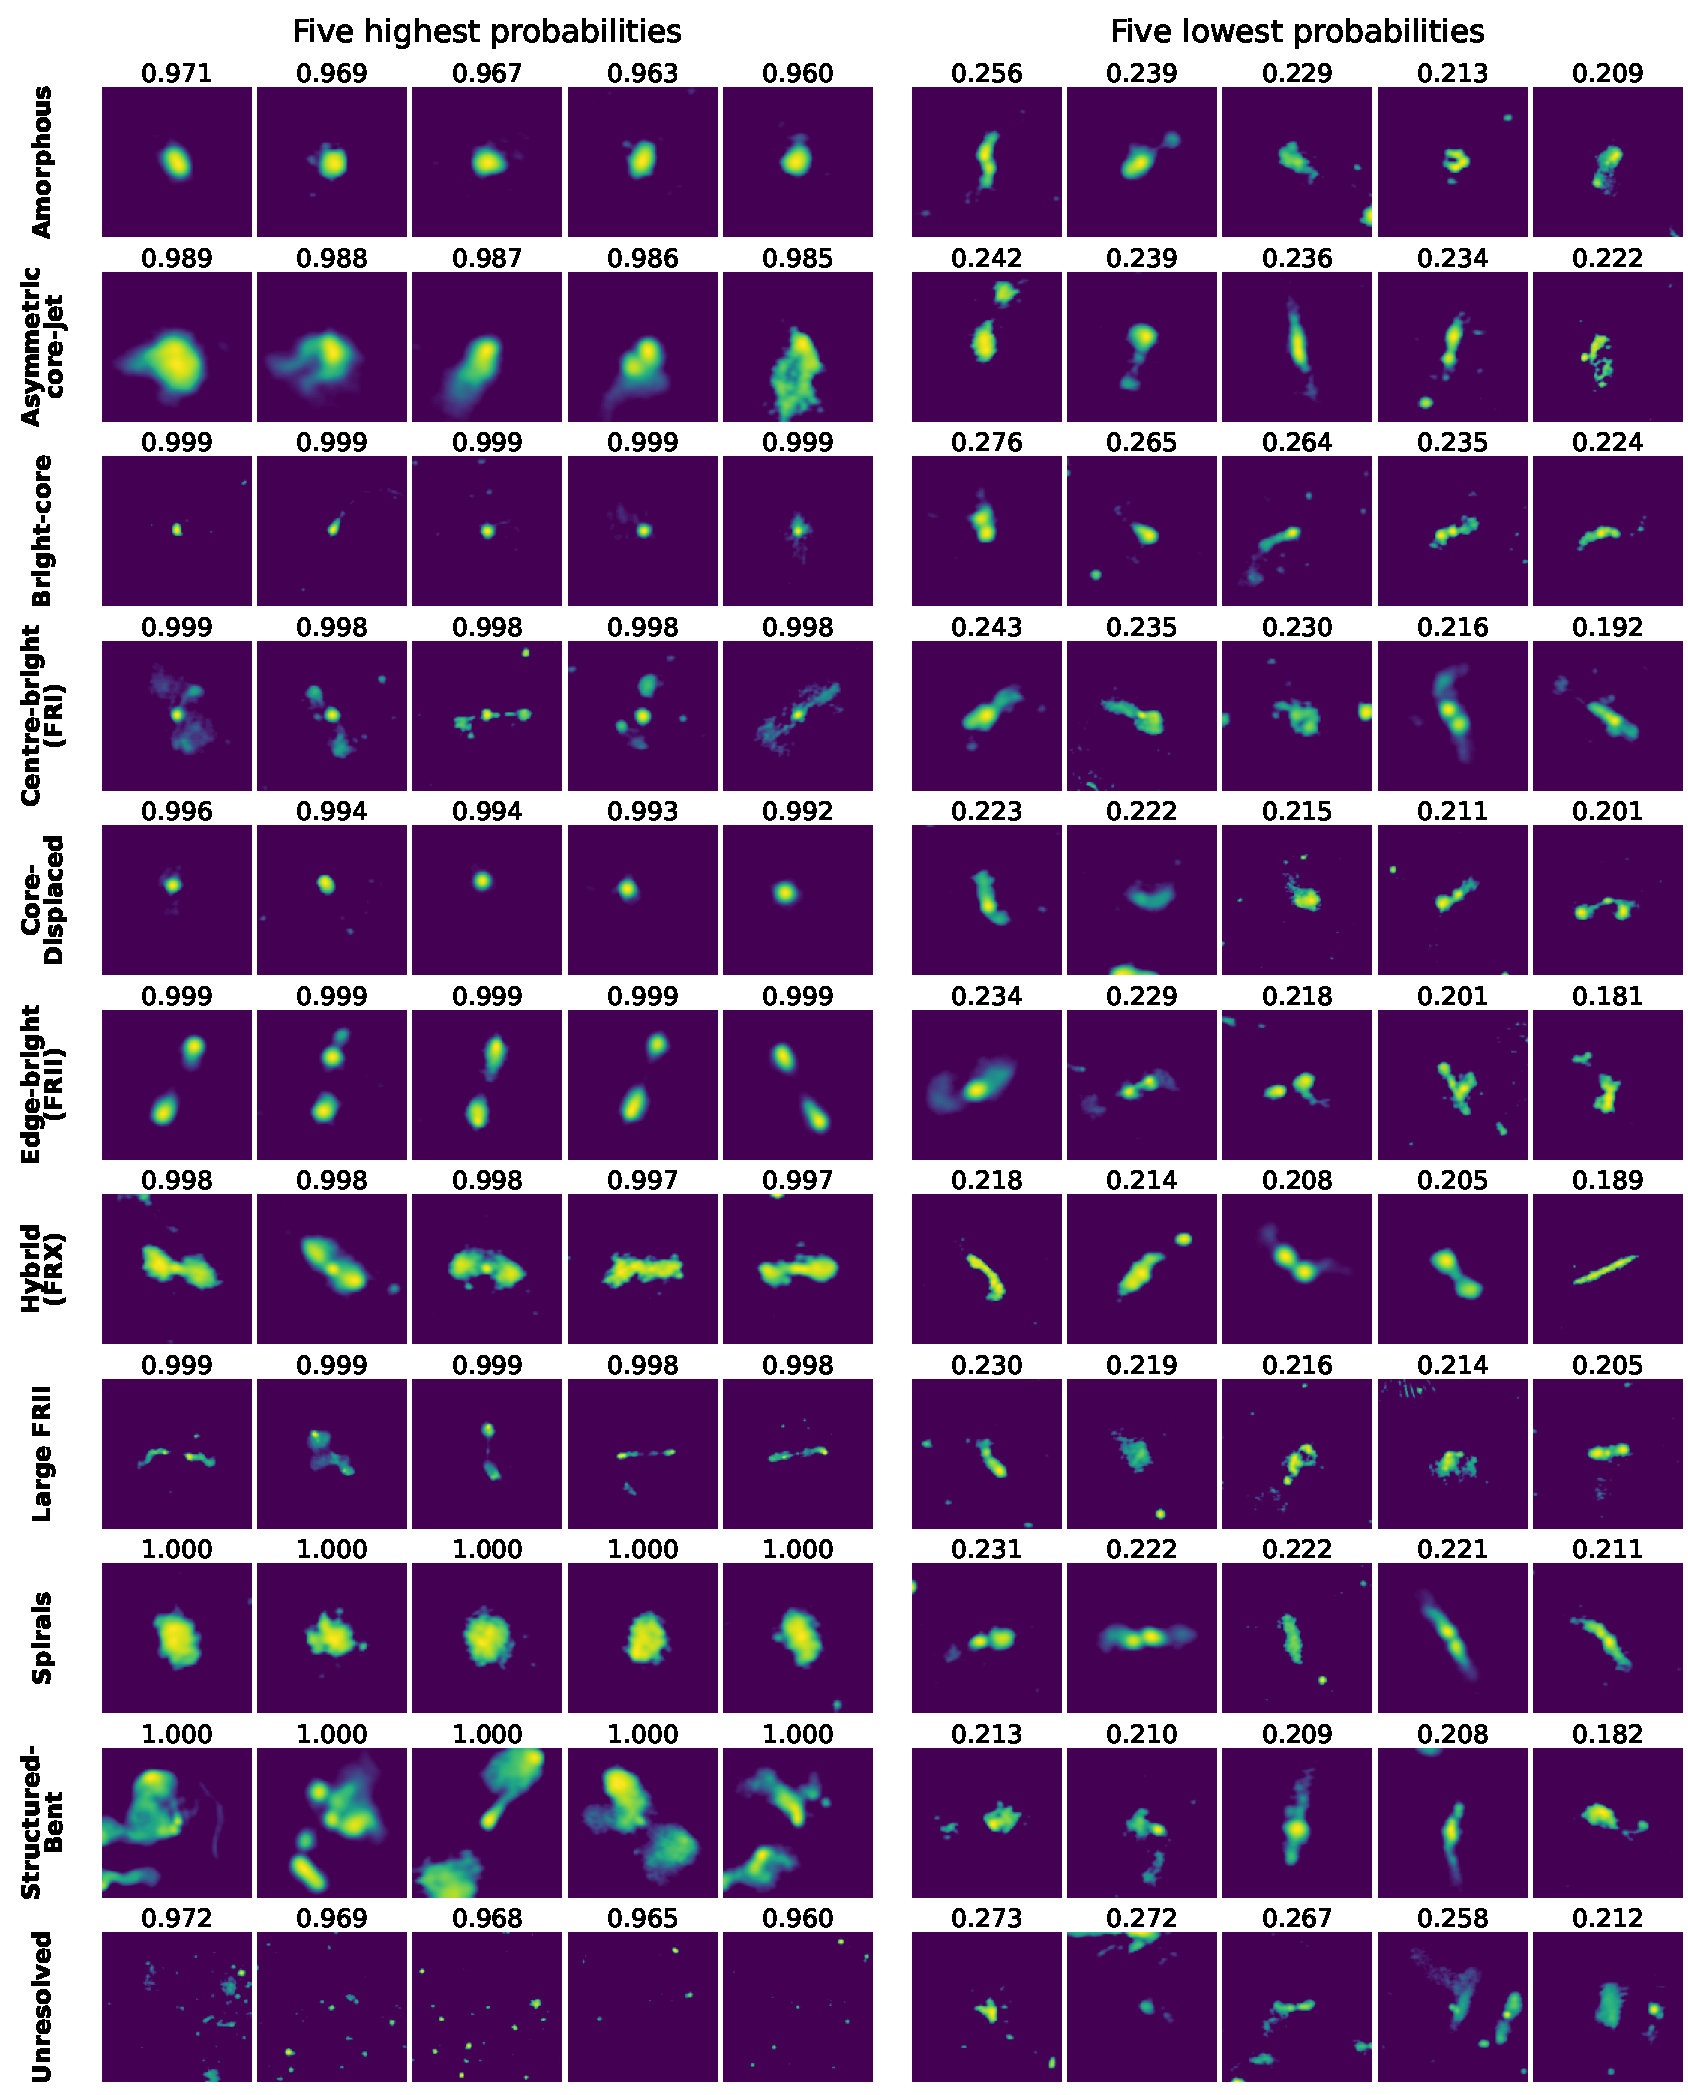
\includegraphics[width=\linewidth]{img/classification_confidence_extremes.pdf}
\caption[Highest- and lowest-confidence examples by class]{Five highest-confidence (left) and five lowest-confidence (right) sources per predicted class. Values above cutouts are ensemble-mean probabilities of the assigned class.}
\label{fig:classification_confidence_extremes}
\end{figure}
\clearpage

\subsubsection{Score distributions and operational bands}

Figure~\ref{fig:srg_dist} shows how the class probabilities and ensemble consistency combine into \(S_\mathrm{RG}\). The radio-galaxy probability mass \(P_\mathrm{RG}\) is concentrated near unity, while the reliability factor \(R\) is more broadly distributed. A large probability mass in the radio-galaxy-like classes therefore does not necessarily produce a high final score.

\begin{figure}[H]
\centering
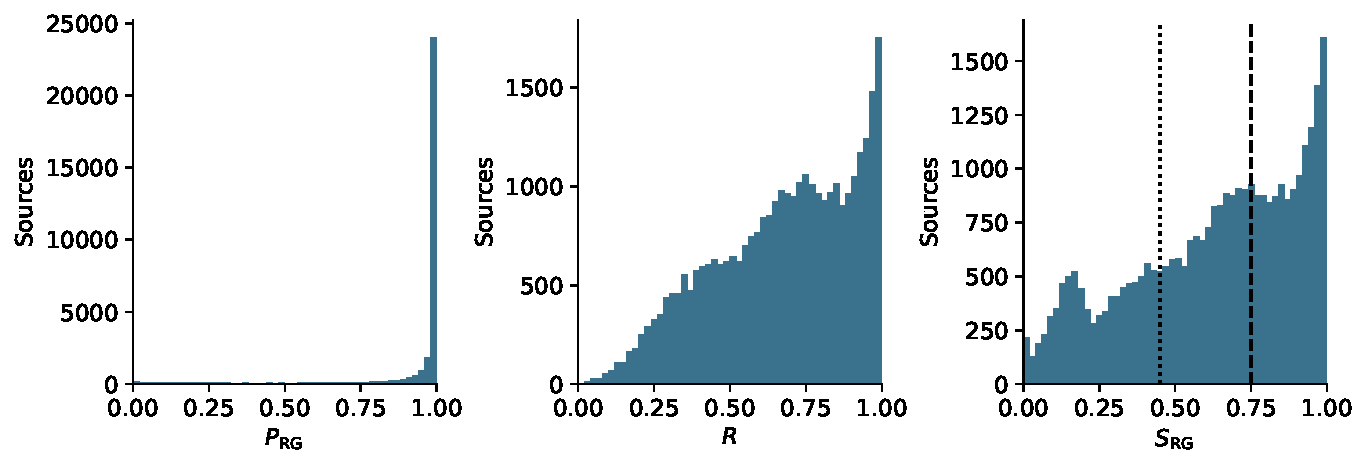
\includegraphics[width=\linewidth]{img/srg_distributions.pdf}
\caption[Full-catalogue score distributions]{Score components for all \(32\,514\) sources. The dashed and dotted lines in the right panel mark \(S_\mathrm{RG}=0.75\) and \(0.45\), respectively.}
\label{fig:srg_dist}
\end{figure}

Table~\ref{tab:srg_bands} divides the catalogue into the adopted high, transitional and low similarity bands. The high-score band is the largest of these review subsets.

\begin{table}[H]
\centering
\begin{tabular}{lrr}
\toprule
Band & Count & Fraction \\
\midrule
High: \(S_\mathrm{RG}\geq0.75\) & 12\,875 & 39.6\,\% \\
Transitional: \(0.45\leq S_\mathrm{RG}<0.75\) & 10\,956 & 33.7\,\% \\
Low: \(S_\mathrm{RG}<0.45\) & 8\,683 & 26.7\,\% \\
\bottomrule
\end{tabular}
\caption[Catalogue membership by score band]{Catalogue membership in the three operational score bands.}
\label{tab:srg_bands}
\end{table}

The class-conditioned distributions in Figure~\ref{fig:srg_class} reflect both the adopted \(G/N\) grouping and the ensemble's support for individual predictions. The non-target classes favour low scores; within \(G\), Bright-core has the highest median and Core-Displaced the lowest. The substantial spread within classes shows why a class assignment alone does not determine the review band.

\begin{figure}[H]
\centering
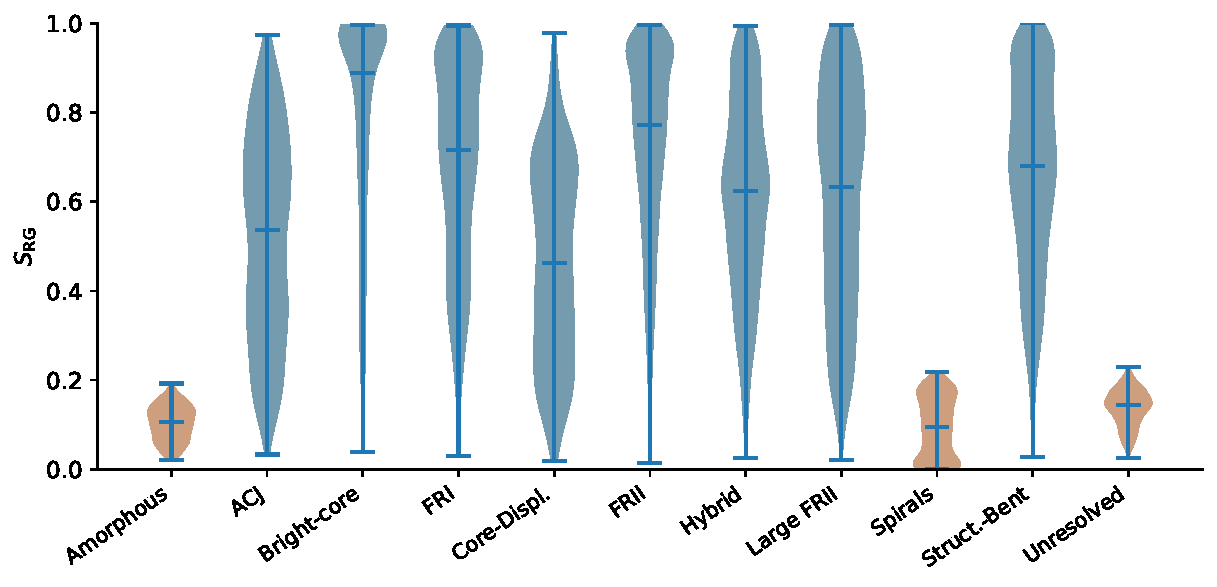
\includegraphics[width=\linewidth]{img/srg_per_class.pdf}
\caption[Similarity-score distributions by predicted class]{Score distributions by ensemble-assigned class. Blue and orange denote the \(G\) and \(N\) groups; central horizontal marks show medians.}
\label{fig:srg_class}
\end{figure}

